\documentclass[../main.tex]{subfiles}

\begin{document}

\chapter{Theoretical Background}
\label{cha:theoretical}

In this chapter the theoretical background for the sensation of fluctuation
strength is presented. First, an introduction to the topic of perceptual
attributes is given. Afterwards, the sensation of fluctuation strength is
addressed, exploring its dependencies on stimulus parameters; most of this
information comes out from the work done by \textcite{Fastl2007Psychoacoustics}.
Next, literature concerning the modeling of fluctuation strength is given.
Finally, several studies expanding upon the basic concepts of fluctuation
strength are presented.

\begin{theoreticalbackground}

\section{Perceptual Attributes}

Perceptual attributes are discernible dimensions in which an auditory event can
be decomposed. They are derived from the physical characteristics of sounds. By
using them the effects of incoming audio events can be understood from a
perceptual point of view. A small overview of the perceptual processes and their
associated perceptual quantities is presented in \Cref{tab:stimsens}, which
summarizes all the perceptual measures, along with their dominant physical
stimuli. Most of the research on perceptual dimensions, except for density,
comes from the ``Munich school'' work of \textcite{Fastl2007Psychoacoustics}.

\begin{table}[ht]
  \centering
  \begin{tabu} to \linewidth{ X X }
    \toprule
    \rowfont\bfseries
    Dominant stimulus dimension & Perceptual parameters \\
    \midrule
    Sound pressure level (dB) & Loudness (sone) \\
    \cmidrule{2-2}
    & Loudness level (phon) \\
    \midrule
    Frequency (Hz) & Critical band rate (Bark) \\
    \cmidrule{2-2}
    & Ratio pitch (mel) \\
    \midrule
    Degree of modulation (\%) & Roughness (asper)\\
    \cmidrule{1-1}
    Modulation frequency (Hz) & \\
    \midrule
    Frequency (Hz) & Sharpness (acum) \\
    \midrule
    Degree of modulation (\%) & Fluctuation strength (vacil) \\
    \cmidrule{1-1}
    Modulation frequency (Hz) & \\
    \midrule
    Spectral components (Pa) & Pitch strength \\
    \cmidrule{2-2}
    & Tonality (tu) \\
    \midrule
    Impulse duration (s) & Subjective duration of impetus (IU) \\
    \midrule
    Sound pressure level (dB) & Density (dasy) \\
    Frequency (Hz) & \\
    \bottomrule
  \end{tabu}
  \caption{Stimuli and sensations~\cite[pp.~70]{Mueller2012Handbook}}
\label{tab:stimsens}
\end{table}

It is important to note that the human auditory system can generate these
perceptual sensations independently of each other, although to understand the
psychological impact of them, for instance the ``pleasantness'' of a given
sound, a bigger context needs to be taken into account. As an example, the
emotions of the listeners can have an important effect on the cognitive
construal of a given sound.

\section{Fluctuation Strength}

Fluctuation strength corresponds to the sensation that arises when a sound
has a slowly varying envelope (i.e., a modulation signal whose frequency is less
than 20~Hz). Fluctuation strength is closely related to roughness, the
difference between the two being the range of modulation frequencies where each
sensation is predominant. In the case of roughness, this range corresponds to
modulation frequency values greater than 20~Hz.

Fluctuation strength can have a significant effect on the pleasantness of sound,
and a particularly clear example of this are alarms, which must have a sharp and
distinctive sound.

The effect of fluctuation strength can be seen as a temporary masking pattern on
the original signal, in which the modulation depth is of utmost importance. This
is also the case for roughness, which resembles fluctuation strength in this
regard.

\subsection{Dependencies of Fluctuation Strength}

The unit used to quantify the sensation of fluctuation strength is the vacil. As
a reference, 1 vacil is defined as the fluctuation strength created by a 1~kHz
tone with a \gls{SPL} of 60~dB, an \gls{AM} envelope of 4~Hz and a modulation
index of 1. The maximum value of fluctuation strength seems to occur for
modulation rates around 4~Hz, regardless of the modulation technique used
(\Cref{fig:flucstrenvmodfreq}).

\begin{figure}[!ht]
  \centering
  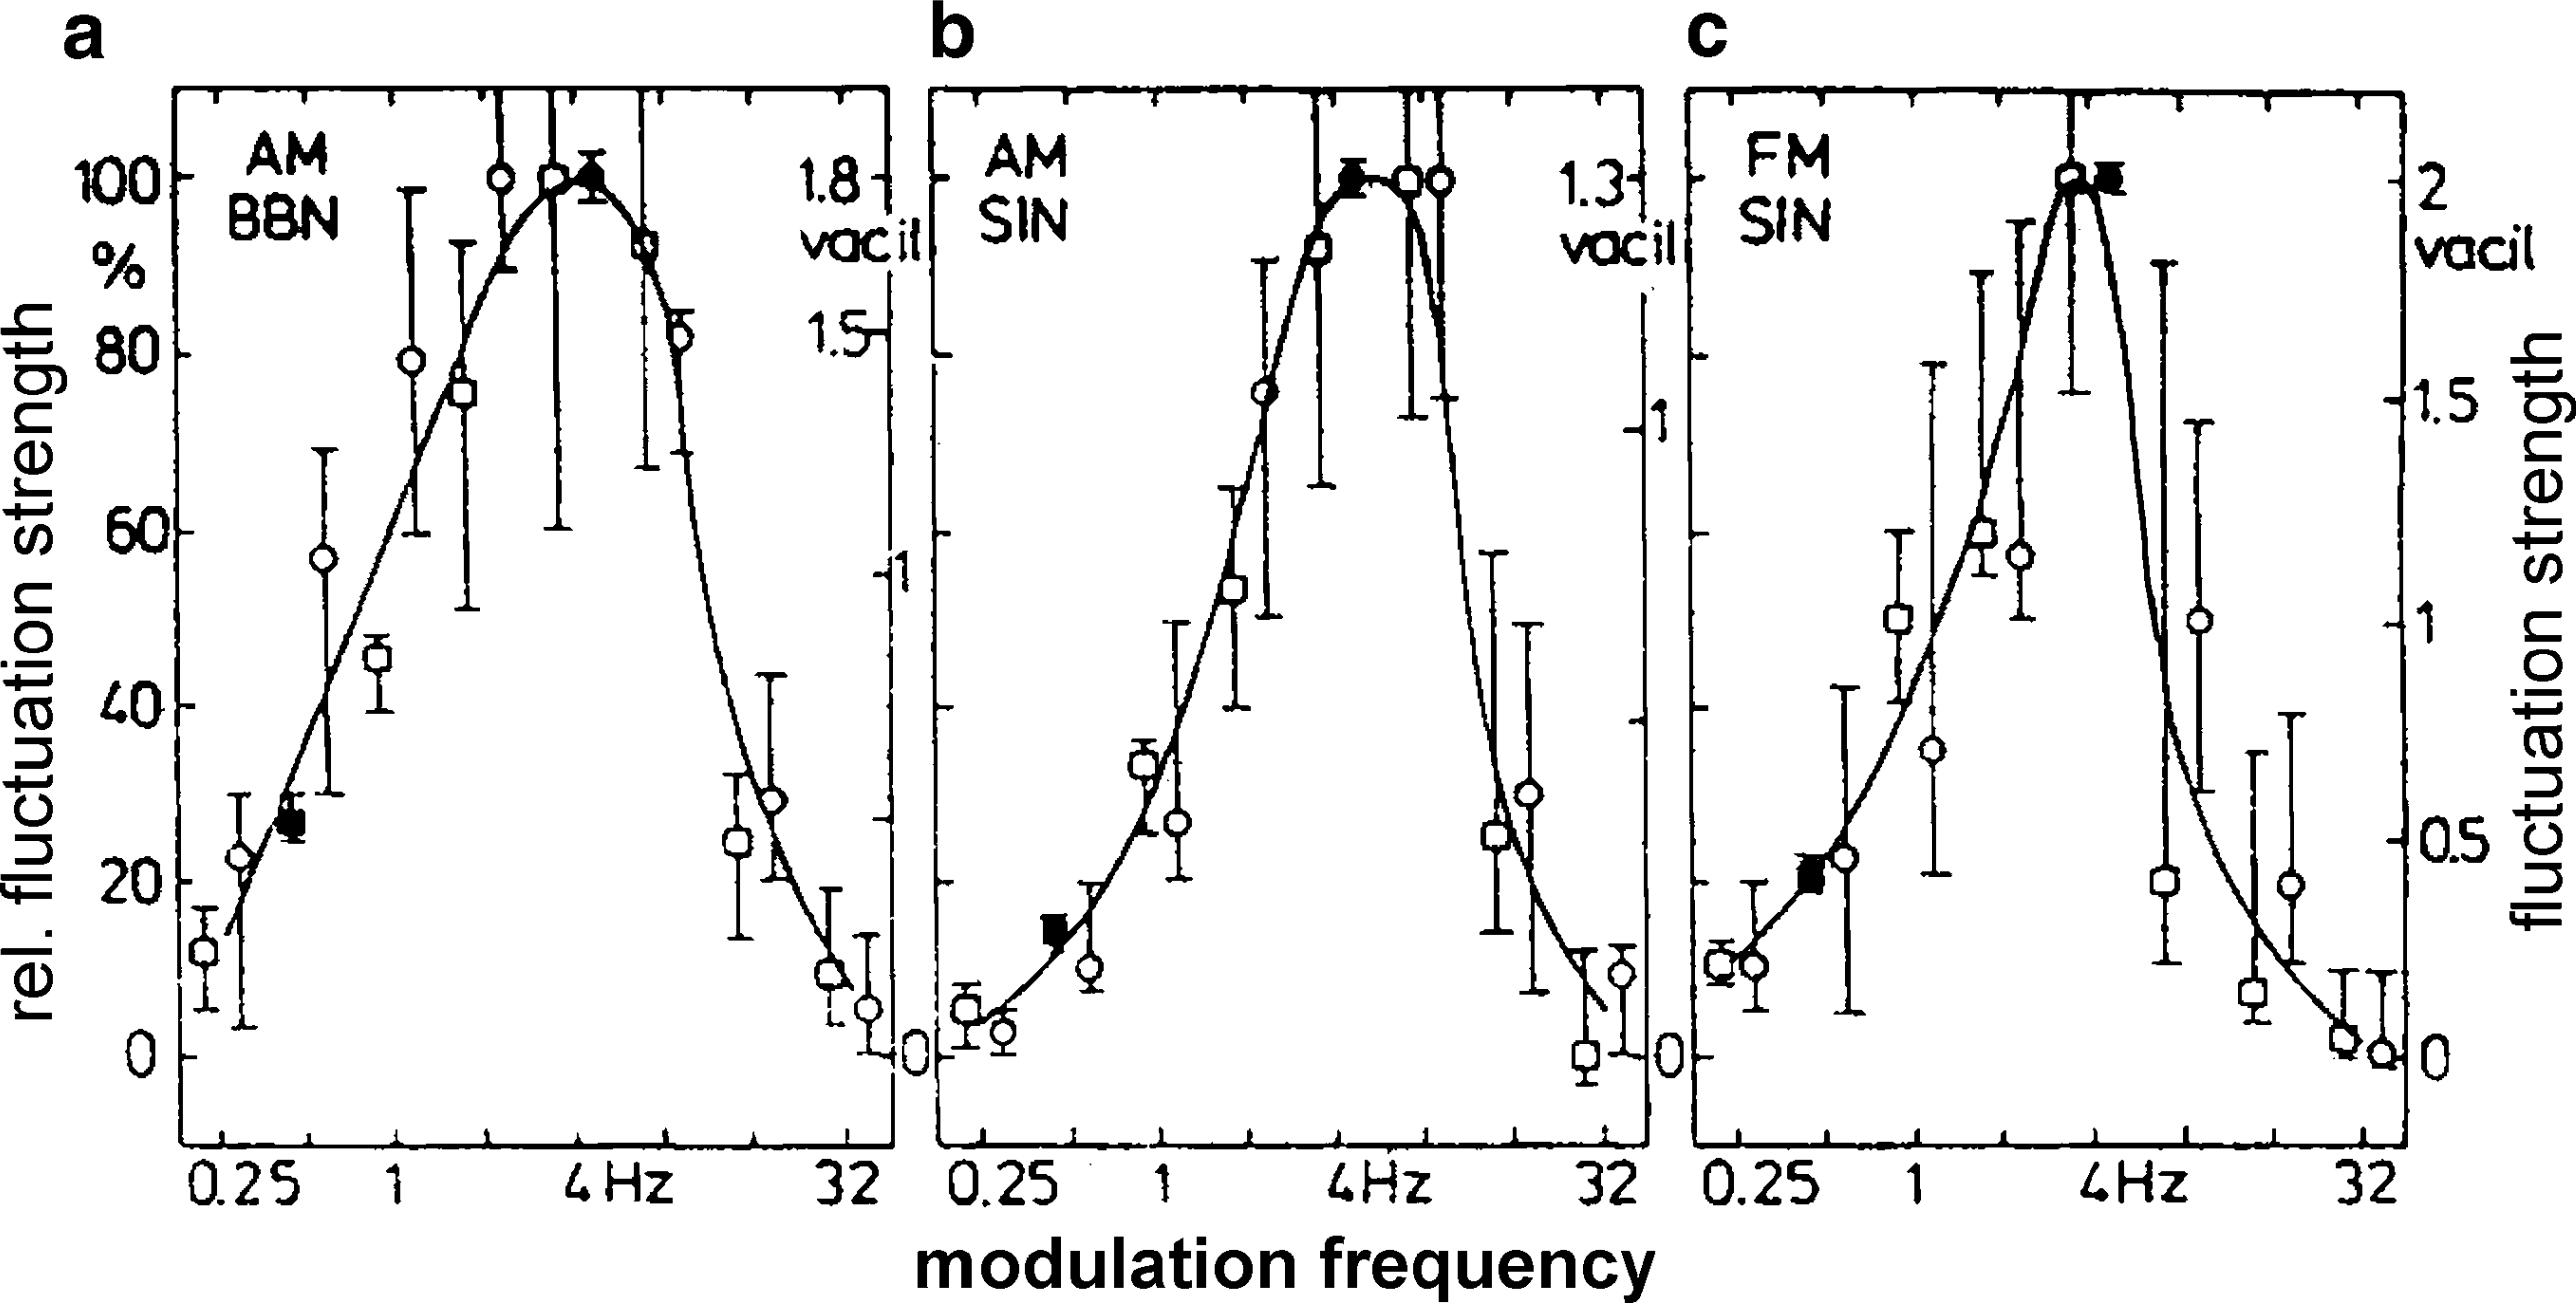
\includegraphics[width=\textwidth]{FluctuationStrengthVsModulationFrequency}
  \caption{Fluctuation strength as a function of modulation frequency for (a)
    amplitude-modulated broad-band noises, (b) amplitude-modulated tones and (c)
    frequency-modulated tones~\cite[pp.~248]{Fastl2007Psychoacoustics}}
\label{fig:flucstrenvmodfreq}
\end{figure}

It seems that a relation between fluctuation strength and speech production
exists, as the normal production rate of syllables during normal conversation
speed is about 4 syllables/second. This coincides with the frequency in which a
maximum value of fluctuation strength occurs (4~Hz).

\Cref{fig:flucstrenvsndpreslvl} shows the relation between \gls{SPL} and
fluctuation strength for two different stimuli, tones and \gls{BBN}, and two
modulation techniques, amplitude modulation and frequency modulation. An
increase in \gls{SPL} entails an increase of fluctuation strength, this being
stronger for the \gls{AM} tones.

\begin{figure}[!ht]
  \centering
  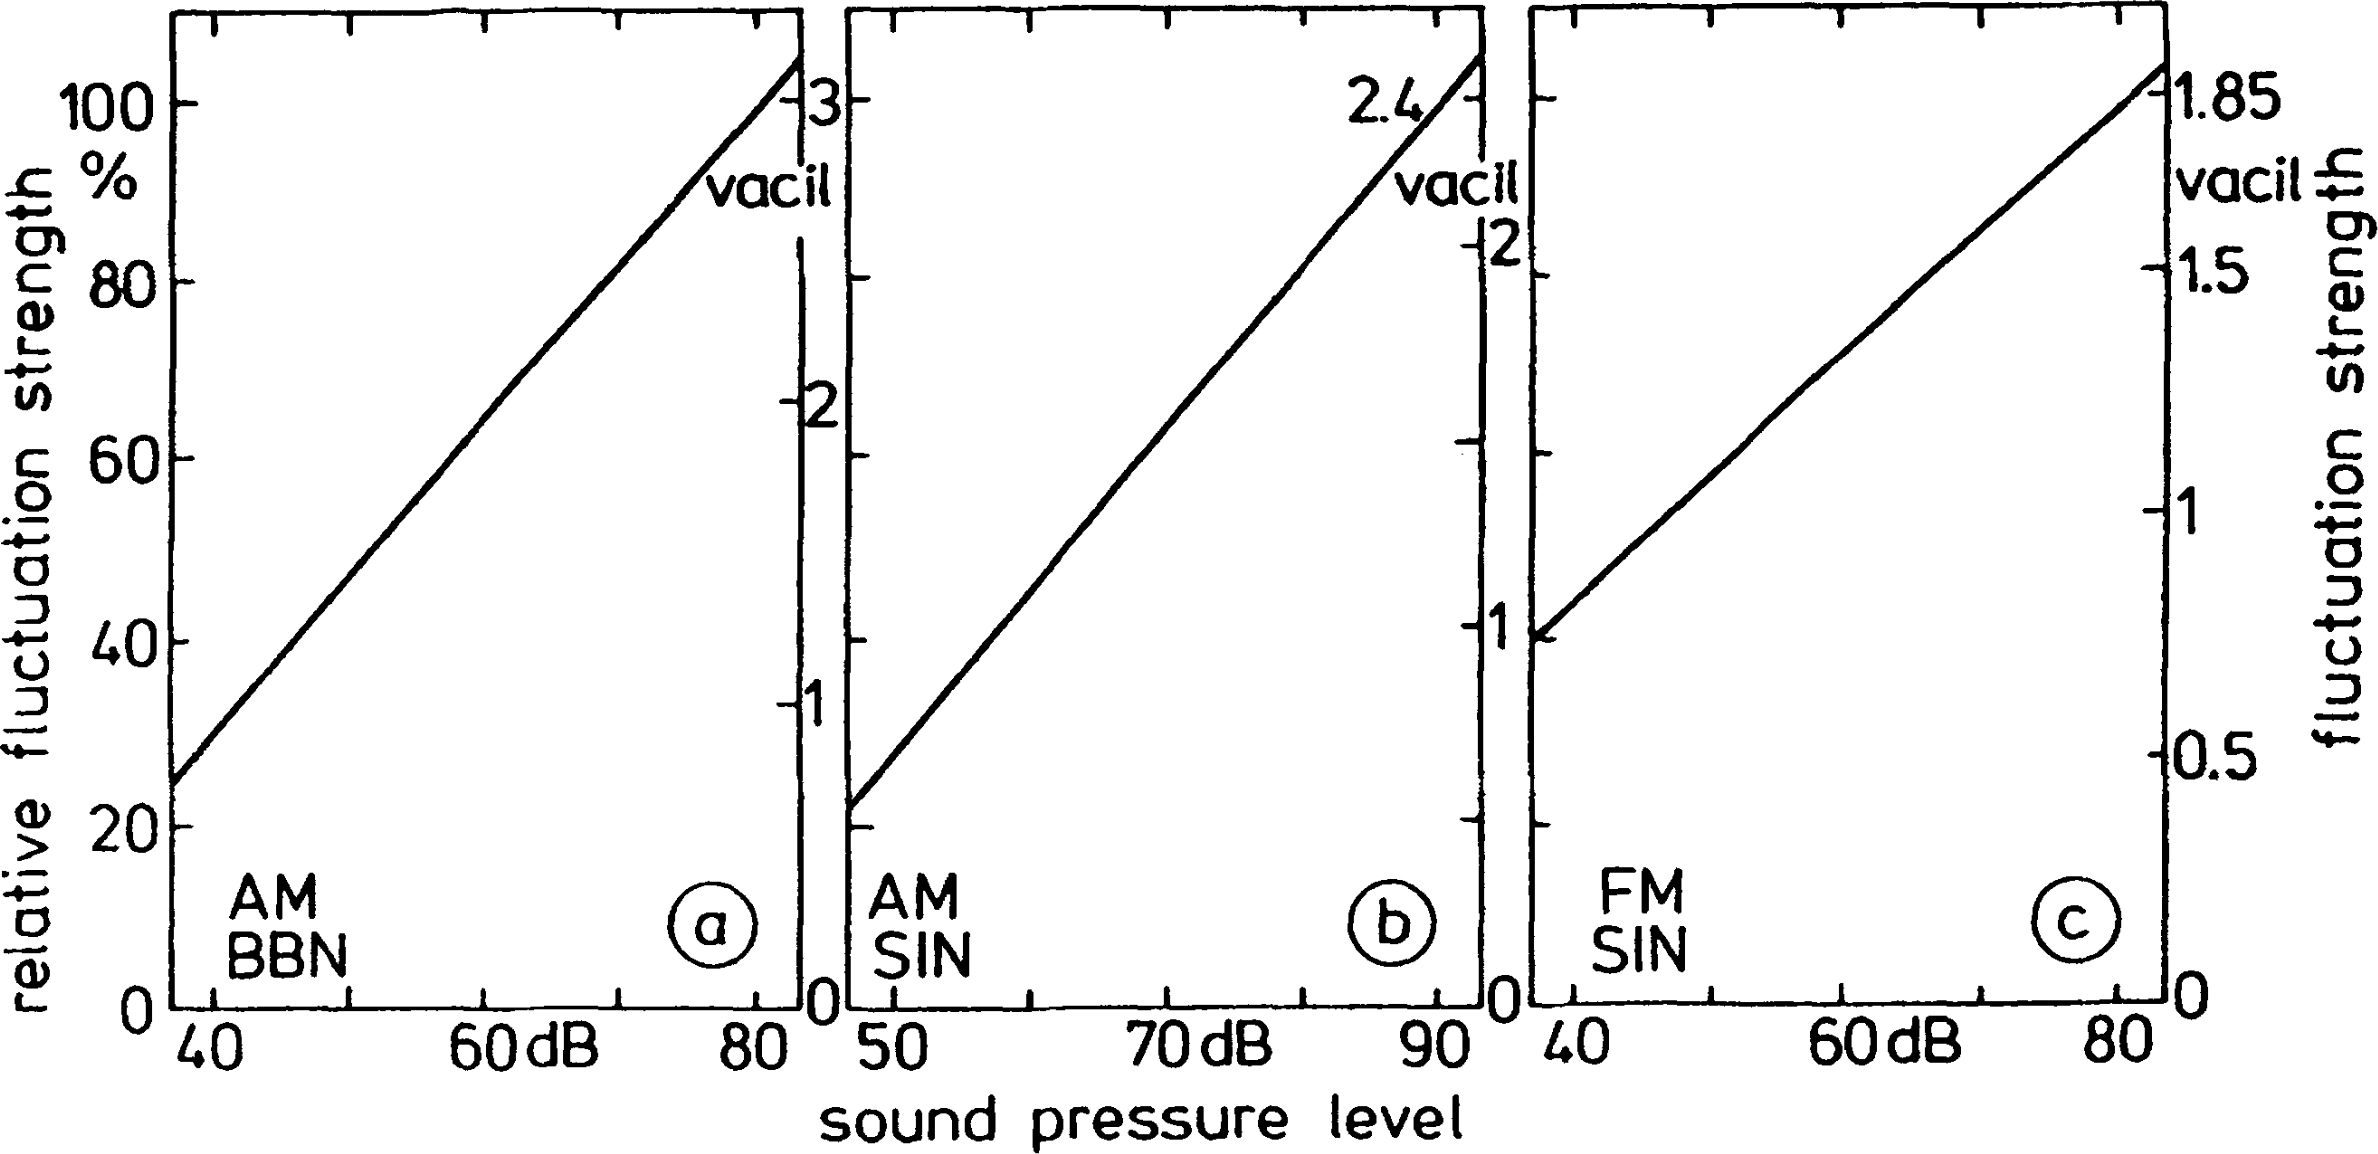
\includegraphics[width=\textwidth]{FluctuationStrengthVsSoundPressureLevel}
  \caption{Fluctuation strength as a function of sound pressure level for (a)
    amplitude-modulated broad-band noises, (b) amplitude-modulated tones and (c)
    frequency-modulated tones; modulation frequency of
    4Hz~\cite[pp.~249]{Fastl2007Psychoacoustics}}
\label{fig:flucstrenvsndpreslvl}
\end{figure}

Next the effect of modulation depth on fluctuation strength is analyzed, shown
in \Cref{fig:flucstrenvsmoddep}. It can be observed that, between 3~dB and 30~dB
the relation between fluctuation strength and modulation depth is somewhat
linear. After reaching a maximum value at around 30~dB, which corresponds to a
modulation factor of 94\%, fluctuation strength remains constant with further
increments of modulation depth.

\begin{figure}[!ht]
  \centering
  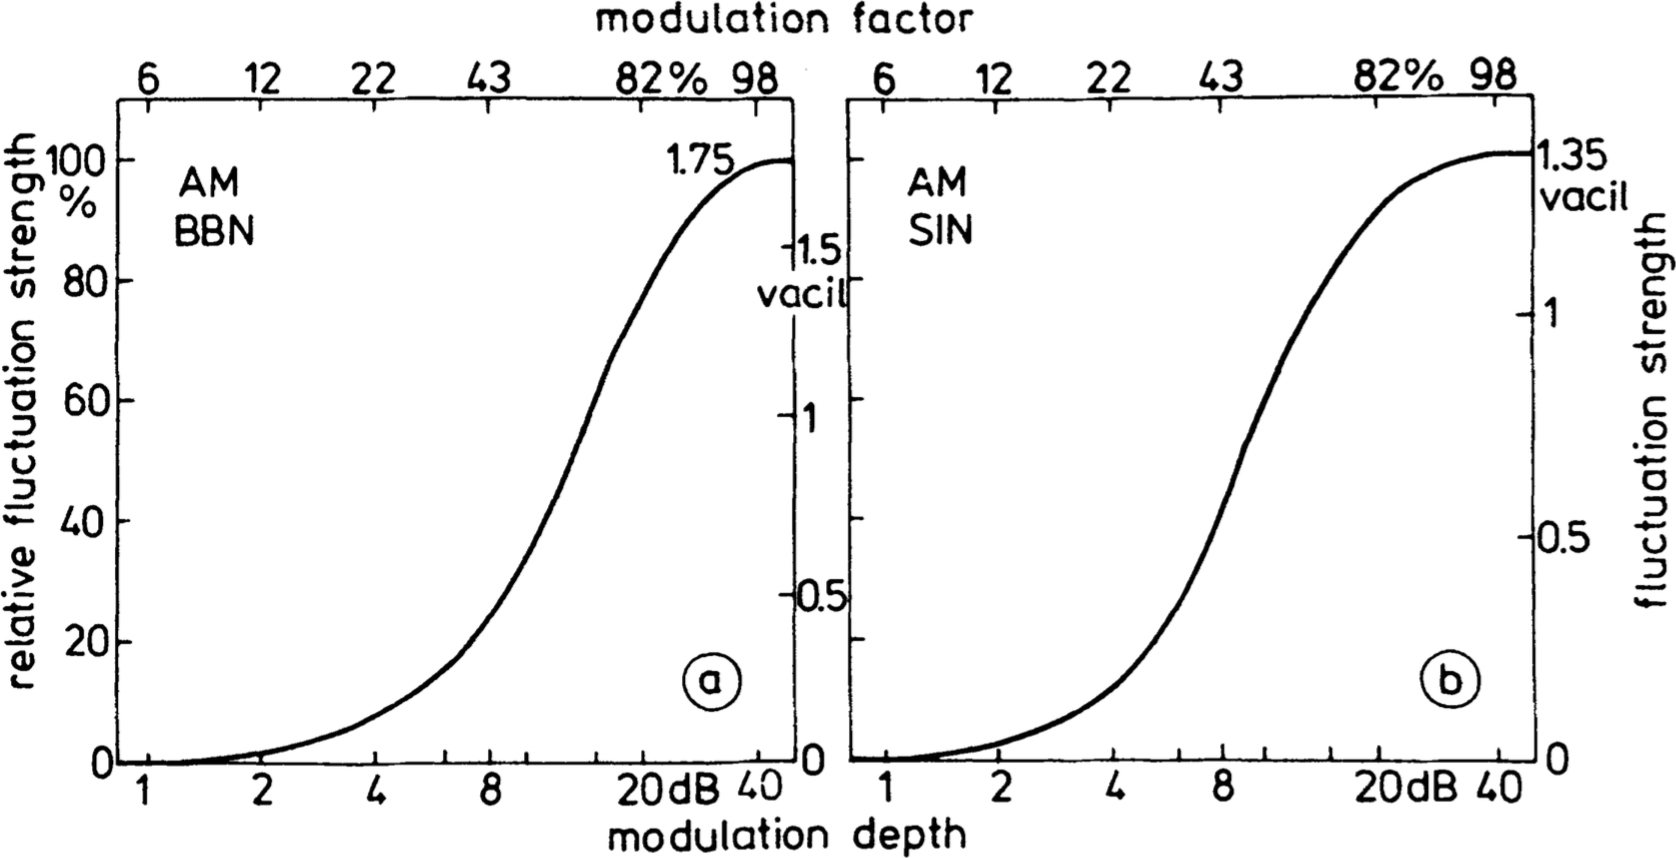
\includegraphics[width=\textwidth]{FluctuationStrengthVsModulationDepth}
  \caption{Fluctuation strength as a function of modulation depth for (a)
    amplitude-modulated broad-band noises of 60~dB SPL and (b)
    amplitude-modulated tones of 70~dB SPL and 1~kHz frequency; both with a
    modulation frequency of 4~Hz~\cite[pp.~249]{Fastl2007Psychoacoustics}}
\label{fig:flucstrenvsmoddep}
\end{figure}

The relation between the center frequency and fluctuation strength is shown in
\Cref{fig:flucstrenvscfreq}. Here a clear difference exists between the type of
modulation used. For \gls{AM} tones there is a small variation in the
fluctuation strength, implying this dependence of fluctuation strength on the
center frequency. For \gls{FM} tones a clear dependence between
both variables exists. For center frequencies below 1~kHz the fluctuation
strength is almost constant; above 1~kHz it experiences a linear decrease until
it fades away at around 8~kHz.

\begin{figure}[!ht]
  \centering
  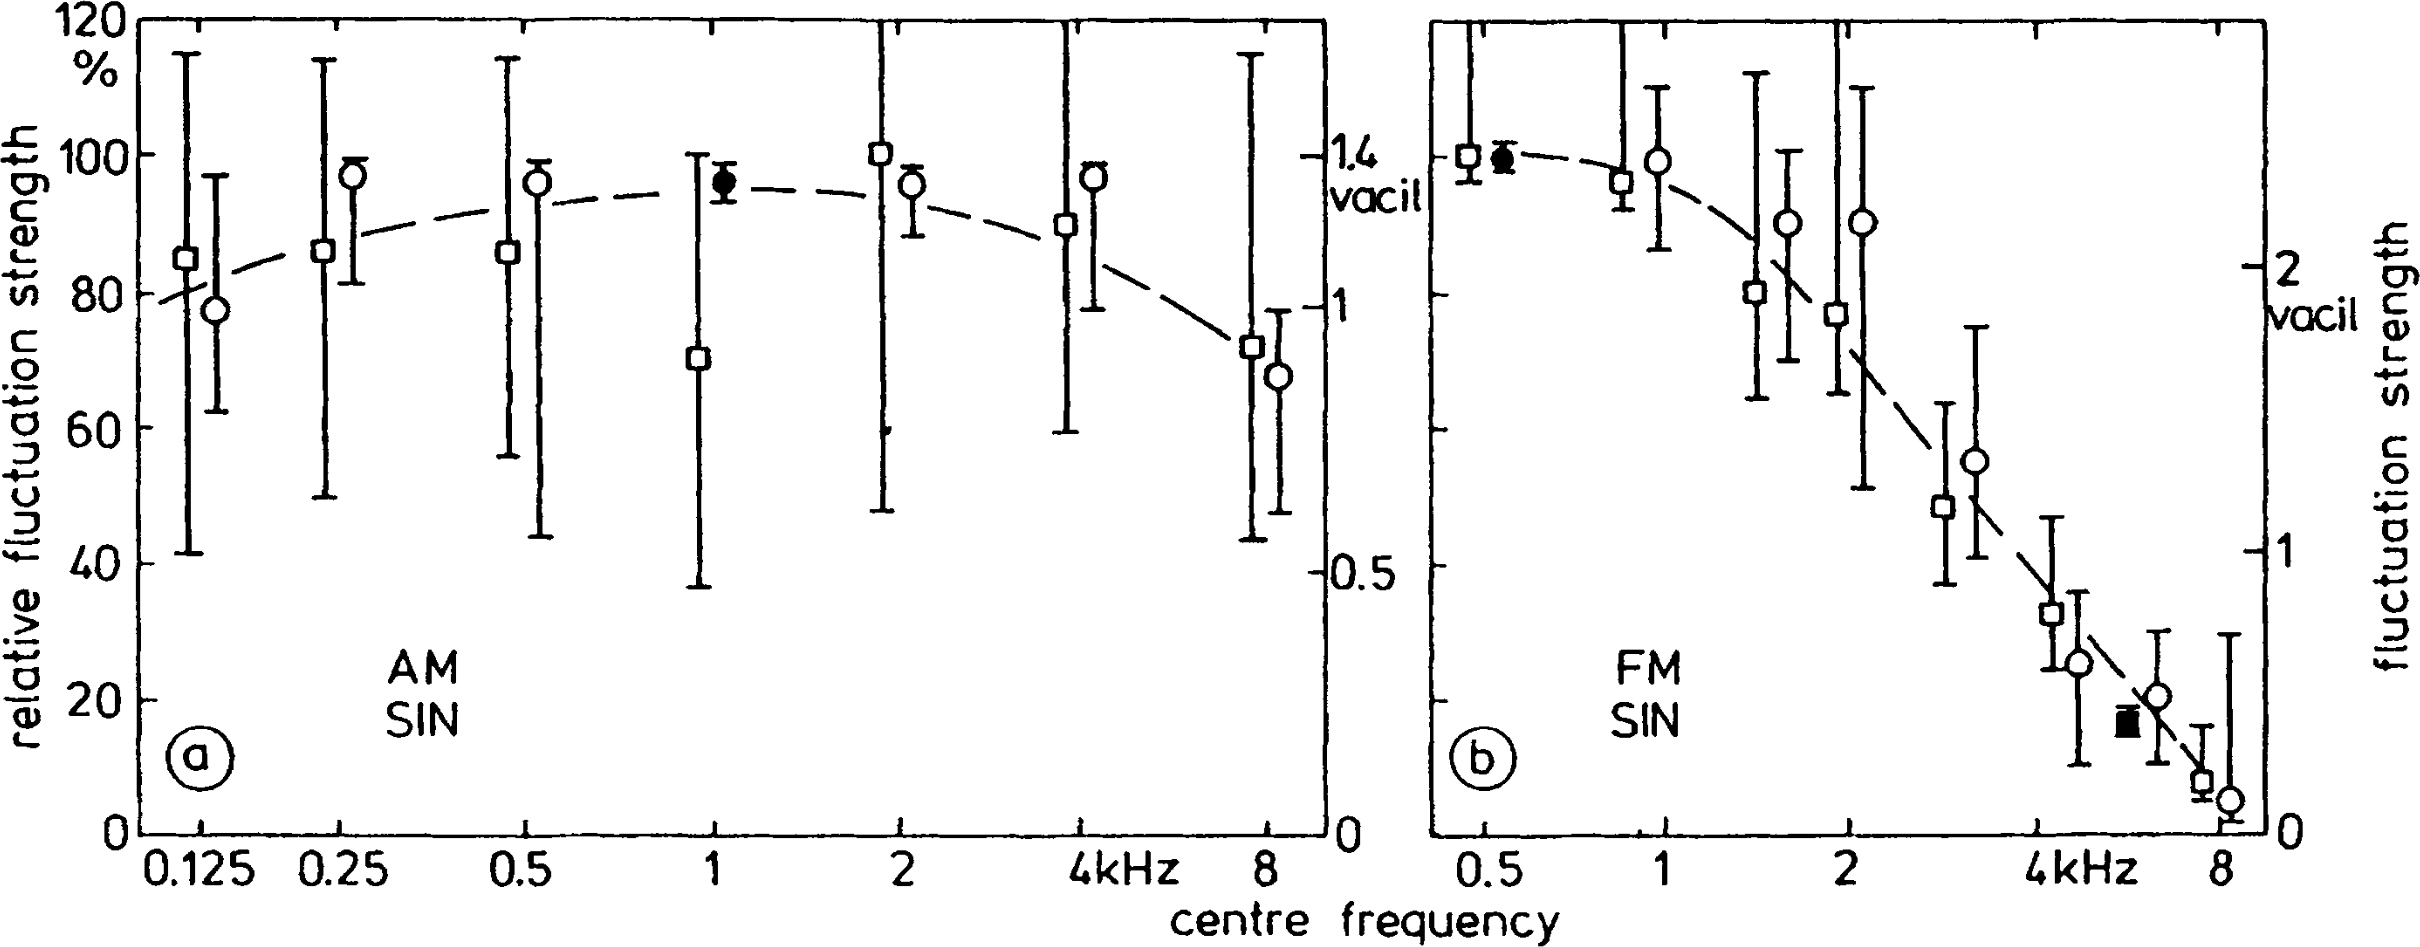
\includegraphics[width=\textwidth]{FluctuationStrengthVsCenterFrequency}
  \caption{Fluctuation strength as a function of center frequency for an
    amplitude-modulated tone of 70~dB SPL, 4~Hz modulation frequency and 40~dB
    modulation depth (a), and a frequency-modulated tone with 70~dB SPL, 4~Hz
    modulation frequency and $\pm200$ Hz frequency
    deviation~\cite[pp. 250]{Fastl2007Psychoacoustics}}
\label{fig:flucstrenvscfreq}
\end{figure}

To understand why this change of fluctuation strength occurs in the case of the
\gls{FM} tones, it is necessary to take into account the excitation patterns
that the modulated sounds cause. The auditory filters are a series of
overlapping bandpass filters that model the frequency selective response of the
auditory system. The excitation pattern refers to the pattern that results as
the outcome of all the precedent stages of the hearing process, being the outer
ear transmission, middle ear transmission, and the auditory filters themselves.

In the case of fluctuation strength, for a \gls{FM} tone with center frequency
of 0.5~kHz and frequency deviation of 200~Hz, the frequency would vary between
300 and 700~Hz. This corresponds to a 3.5~Bark interval. For a tone with center
frequency of 8~kHz and frequency deviation of also 200~Hz these values would be
7.8~kHz and 8.2~kHz, leading to a 0.2~Bark interval. For both \gls{FM} tones the
range of frequency is constant of a Hertz scale, i.e. 400~Hz. The proportion
between these two is 17.5, which seems to be also the proportion between the
relative fluctuation strength for these two frequencies. Thus, this leads to the
idea that fluctuation strength can be explained in terms of the excitation
patterns that present themselves across the auditory filters.

\Cref{fig:flucstrenvsfreqdev} shows the relation between fluctuation strength
and frequency deviation. It can be seen that, for frequencies above 20~Hz, there
is a linear increase of fluctuation strength with frequency deviation.

\begin{figure}[!ht]
  \centering
  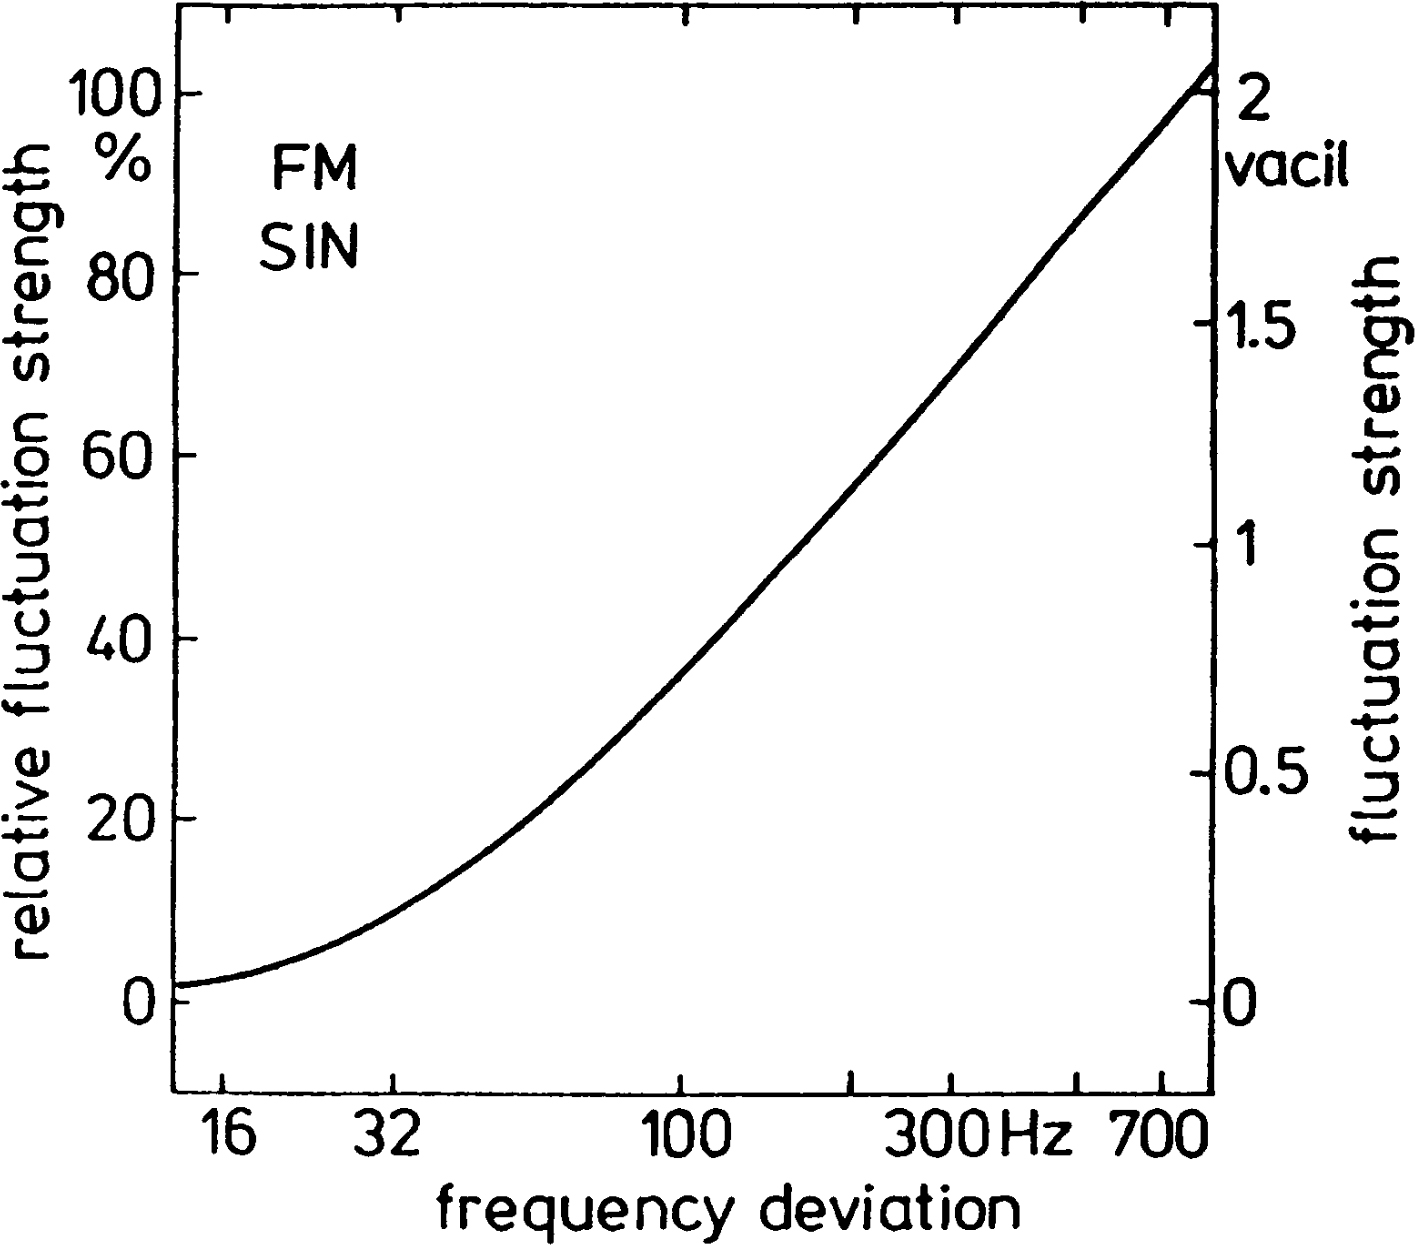
\includegraphics[height=8cm]{FluctuationStrengthVsFrequencyDeviation}
    \caption{Fluctuation strength as a function of frequency deviation for a
      tone with 70~dB SPL, 1.5~kHz center frequency and a modulation frequency
      of 4~Hz~\cite[pp. 251]{Fastl2007Psychoacoustics}}
\label{fig:flucstrenvsfreqdev}
\end{figure}

Another variable that affects fluctuation strength is the modulation index $h$
(also called modulation factor $m$). It is defined differently according to the
type of modulation used:
\begin{itemize}
  \item For \gls{AM} signals is the ratio between the modulating signal
    amplitude $M$ and the carrier signal amplitude $A$,
      \begin{equation}
        x_{am} = [1+h \cdot \sin(2\pi f_m t)]\cdot A \cdot \sin(2\pi f_c t)
      \end{equation}
      \begin{equation}
        h=\frac{M}{A}
      \end{equation}
  \item For \gls{FM} signals is the ratio between the maximum frequency
    deviation in the carrier signal ($\Delta f$) and the maximum frequency
    component of the modulating signal ($f_m$),
      \begin{equation}
        x_{fm} = A \cdot \sin[2\pi f_c t + h \cdot \sin(2 \pi f_m t)]
      \end{equation}
      \begin{equation}
        h=\frac{\Delta f}{f_m}
      \end{equation}
\end{itemize}

\Cref{fig:flucstrensnds} compares the fluctuation strength of several sounds,
whose physical characteristics are described in \Cref{tab:flucstrensnds}. The
sounds that present the largest values of fluctuation strength (sounds 1 and 2)
excite a large range of frequencies and therefore more than one auditory filter.
As so, it can be said that fluctuation strength sums across critical bands.

\begin{figure}[!ht]
  \centering
  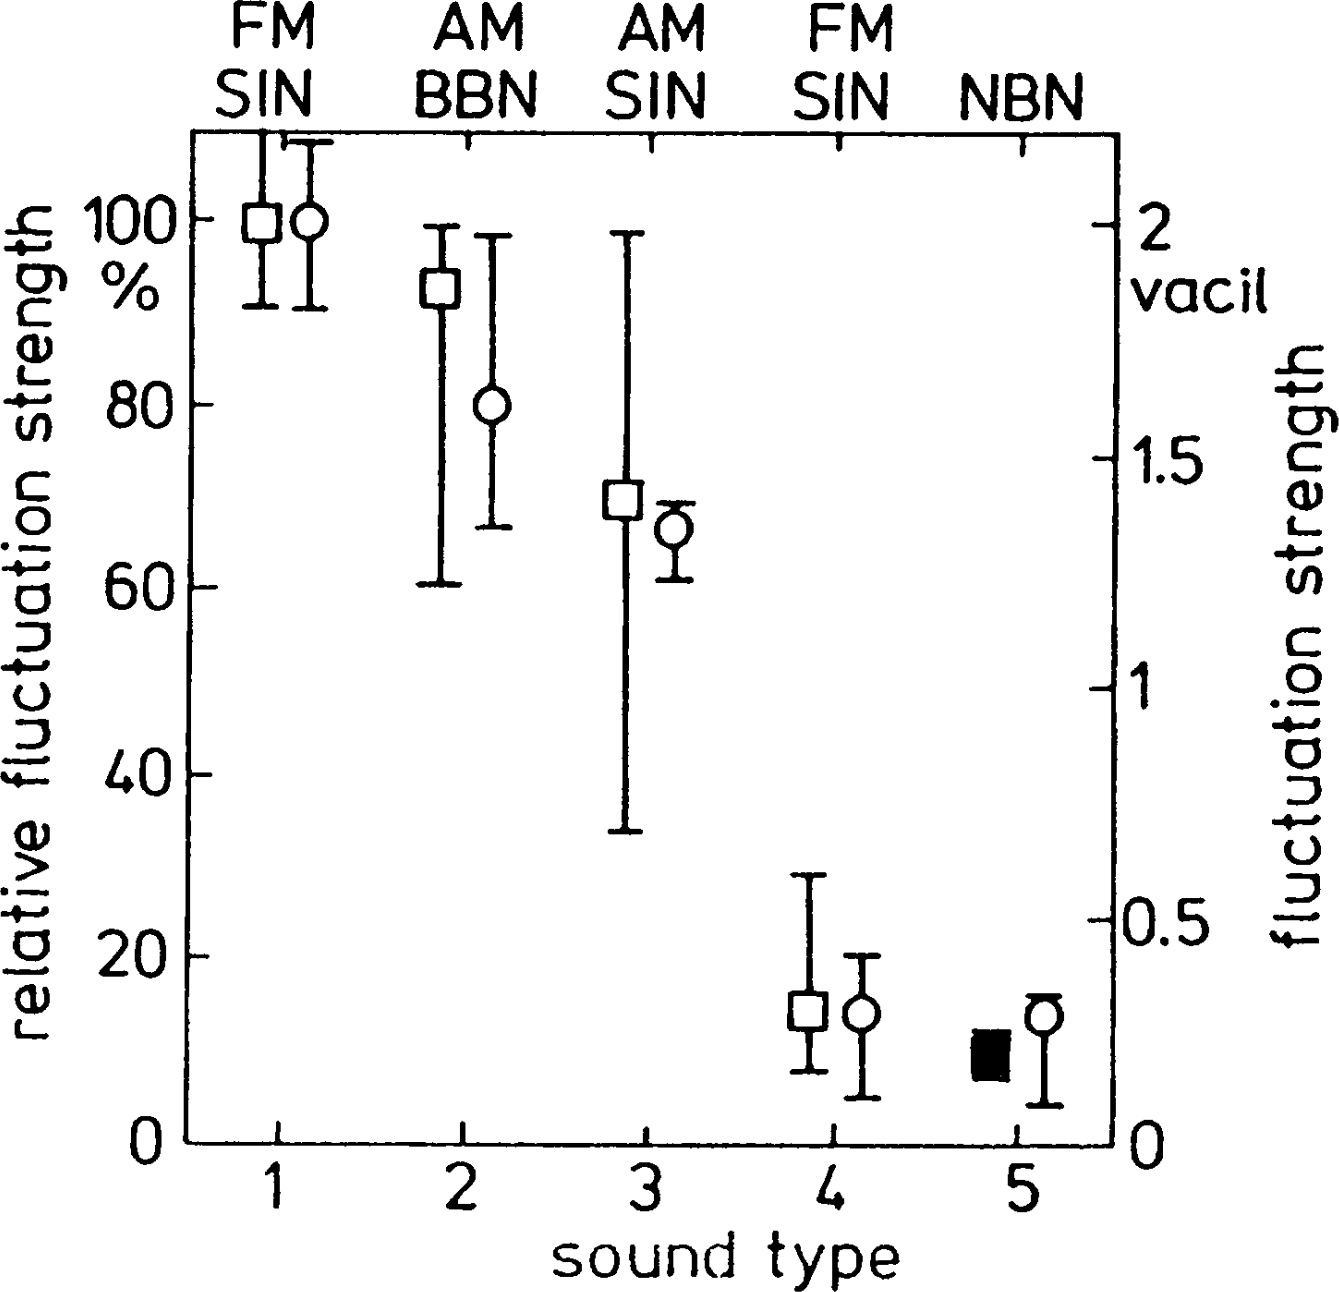
\includegraphics[height=8cm]{FluctuationStrengthSounds}
  \caption{Fluctuation strength of sounds 1--5 as described in
    \Cref{tab:flucstrensnds}~\cite[pp. 252]{Fastl2007Psychoacoustics}}
\label{fig:flucstrensnds}
\end{figure}

\begin{table}[!ht]
  \centering
  \begin{tabu} to \linewidth{ lXXXXX }
    \toprule
    Sound & 1 & 2 & 3 & 4 & 5 \\
    \midrule
    Abbreviation & FM & AM & AM & FM & \\
    & SIN & BBN & SIN & SIN & NBN \\
    Frequency [Hz] & 1500 & --- & 2000 & 1500 & 1000 \\
    Level [dB] & 70 & 60 & 70 & 70 & 70 \\
    Modulation frequency [Hz] & 4 & 4 & 4 & 4 & --- \\
    Modulation depth [dB] & --- & 40 & 40 & --- & --- \\
    Frequency deviation [Hz] & 700 & --- & --- & 32 & --- \\
    Bandwidth [Hz] & --- & 16000 & --- & --- & 10 \\
    \bottomrule
  \end{tabu}
  \caption{Physical data of sounds
    1--5~\cite[pp. 253]{Fastl2007Psychoacoustics}}
\label{tab:flucstrensnds}
\end{table}

\subsection{Models of Fluctuation Strength}

A basic model for fluctuation strength (proposed by
\textcite[pp.~254]{Fastl2007Psychoacoustics}) based on the temporal variation of
the masking pattern of the sound to analyze is shown in
\Cref{fig:flucstrenmodel}, where the temporal variation of the amplitude of the
masking pattern, also called temporal masking depth, is denoted by the magnitude
$\Delta L$. The inverse of the time difference between peaks corresponds to the
\gls{f_m}.

\begin{figure}[!ht]
  \centering
  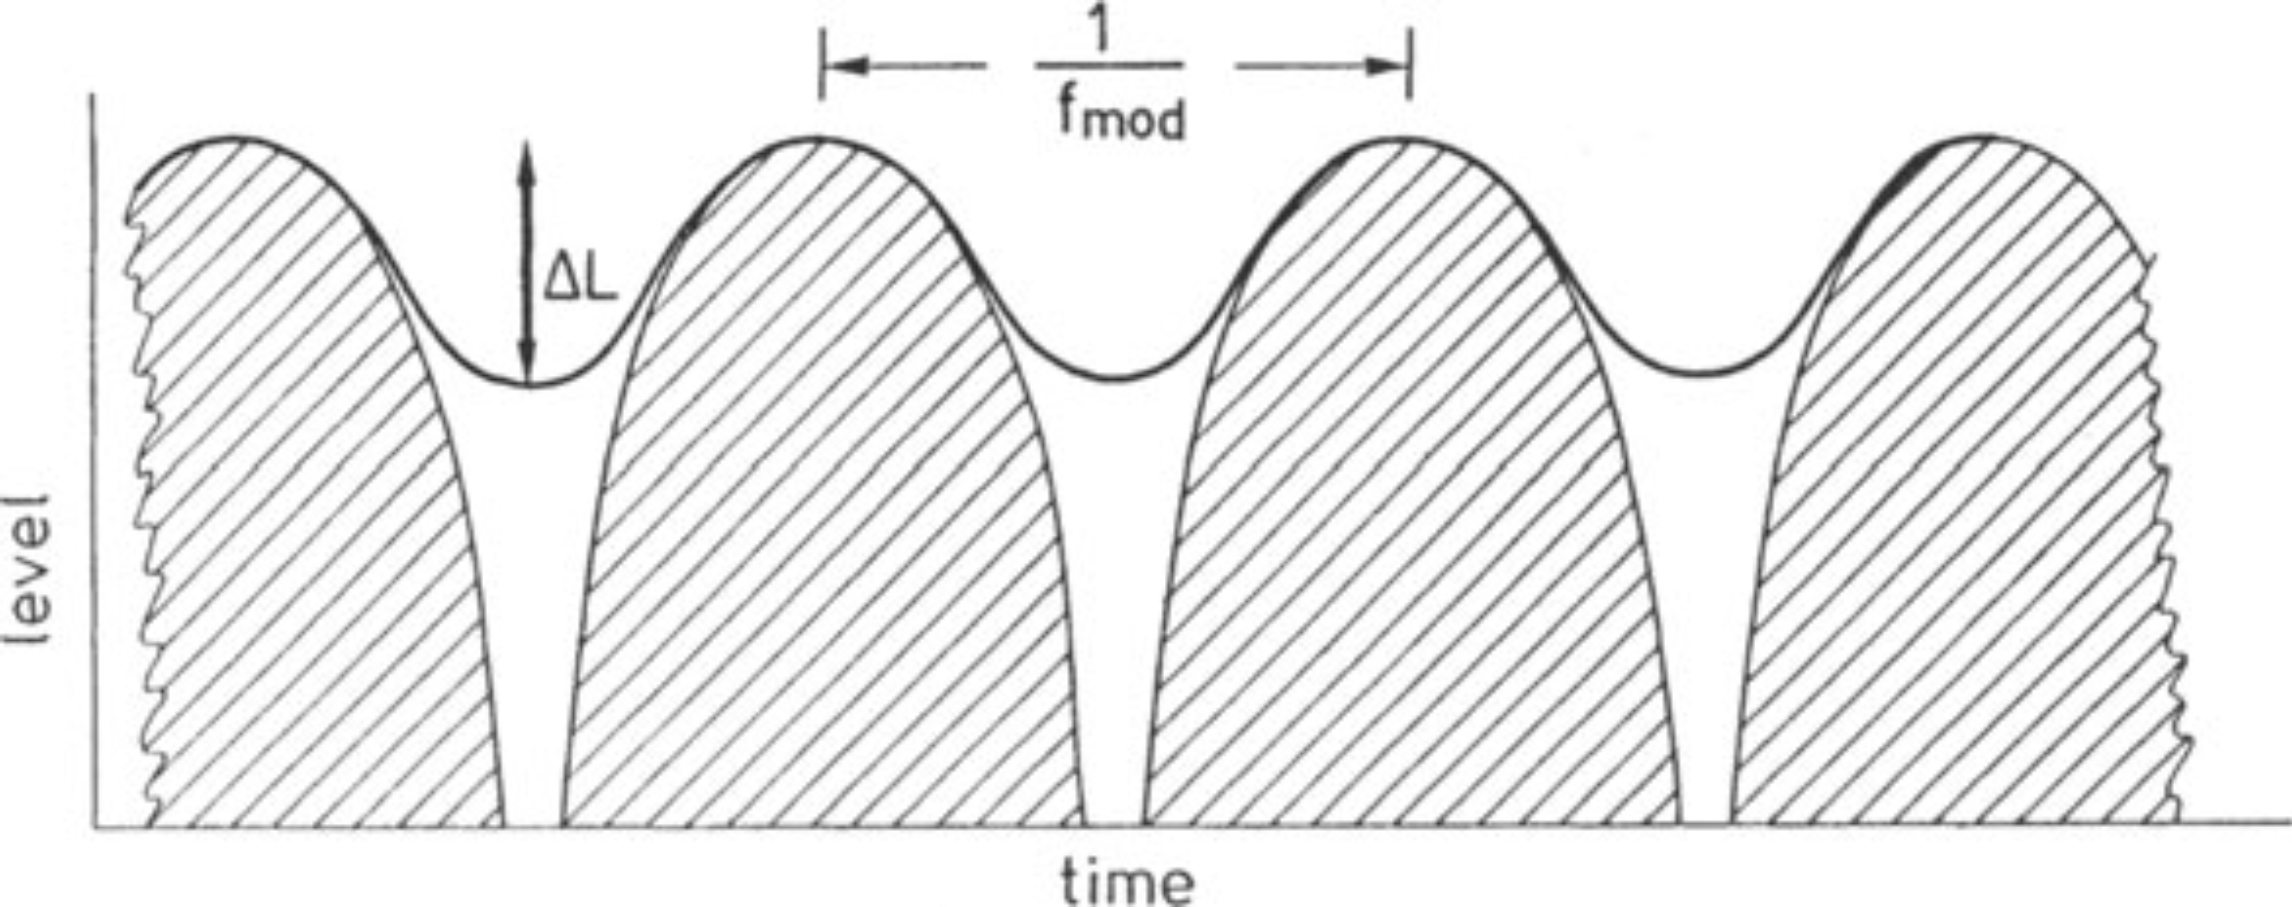
\includegraphics[width=\textwidth]{FluctuationStrengthModel}
  \caption{Model of fluctuation
    strength~\cite[pp. 254]{Fastl2007Psychoacoustics}}
\label{fig:flucstrenmodel}
\end{figure}

\Cref{eq:flucstrentempmaskmodfreq} shows the relationship between fluctuation
strength $F$, temporal masking depth $\Delta L$ and modulation frequency
$f_{m}$, where the importance of the 4 Hz frequency is emphasized.

\begin{equation}
  F \sim \frac{\Delta L}{(f_{m}/4\text{ Hz}) + (4\text{ Hz}/f_{m})}
  \label{eq:flucstrentempmaskmodfreq}
\end{equation}

It should be noted that there is a dependency between the temporal masking depth
$\Delta L$ and the modulation frequency depending on the type of stimuli. In the
case of \gls{BBN} stimuli, the temporal masking depth is largely independent of
modulation frequency~\cite[pp.~254]{Fastl2007Psychoacoustics}, whereas for
amplitude and frequency modulated tones these two variables are dependent on
each other, due to the nonlinearity of the upper slope in the masking pattern.
This effect being the strongest for \gls{FM} stimuli. In order to address this,
when modeling the fluctuation strength for these tones not a single
$\Delta L$ value is taken, but instead it is integrated across the critical-band
rate scale.

The resulting temporal masking pattern for several values of modulation
frequency is shown in \Cref{fig:flucstrenmasking}. It can be seen that, as the
modulation frequency increases, the temporal masking depth decreases. This leads
to the idea that, although fluctuation strength presents a bandpass response
with respect to modulation frequency, the temporal masking reveals a low pass
characteristic. It can be considered that the temporal masking depth decreases
linearly with modulation frequency, as shown on \Cref{fig:flucstrenmasking}.

\begin{figure}[!ht]
  \centering
  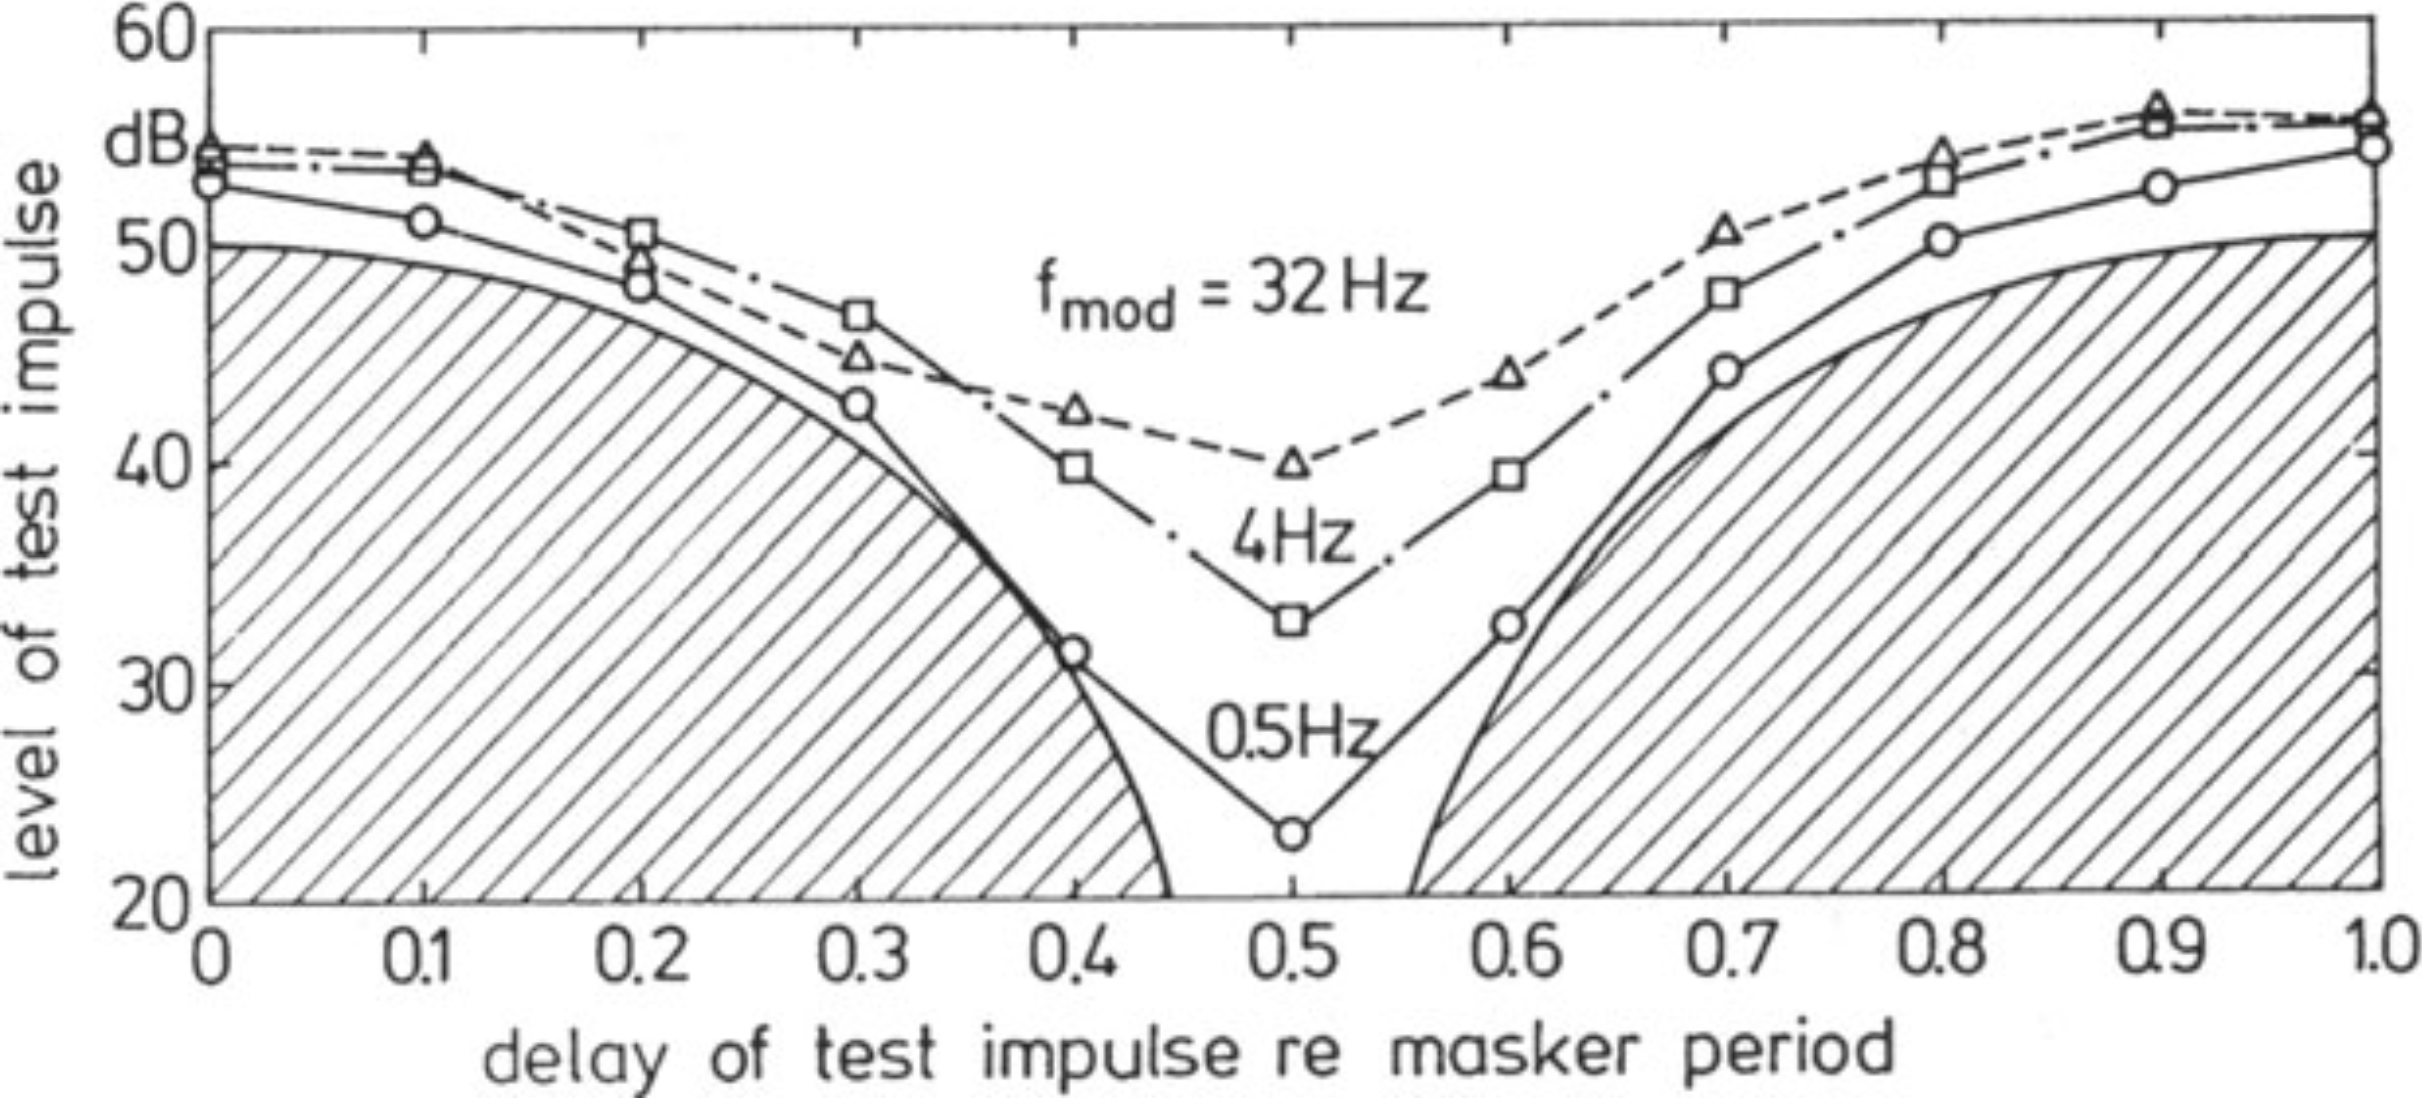
\includegraphics[width=\textwidth]{FluctuationStrengthTemporalMasking}
  \caption{Temporal masking pattern for an amplitude-modulated broad-band
    noise~\cite[pp. 255]{Fastl2007Psychoacoustics}}
\label{fig:flucstrenmasking}
\end{figure}

The modeling based on the temporal masking property, proposed by
\citeauthor{Fastl2007Psychoacoustics}, poses difficulties when its
implementation details are addressed. Furthermore, to our knowledge, there is
not a publicly available implementation for any given model of fluctuation
strength up to this date. There are, however, implementation models when it
comes to roughness, a sensation that it was already mentioned as being similar
to fluctuation strength regarding its physical characteristics. The most
prominent of these models is the one developed by
\textcite{daniel1997psychoacoustical}, which is based on the dependency of
roughness on modulation depth, shown in \Cref{eq:R}.

\begin{equation}
  R \sim m^p
  \label{eq:R}
\end{equation}

In order to obtain a roughness value from a given sound, the model first
decomposes the incoming signal into excitation patterns, using a critical
filterbank composed of 47 channels. Each excitation pattern is then band-pass
filtered, to account for the dependence of roughness on modulation frequency.
After this, an estimate of the modulation depth present in the signal is
calculated, using a generalized modulation depth function \Cref{eq:genmod}.

\begin{equation}
  {m_i}^* = \tilde{h}_{BP,i}(t)/h_{0,i}
  \label{eq:genmod}
\end{equation}
where $\tilde{h}_{BP,i}(t)$ is the \gls{RMS} value of the band-pass filtered
signal and $h_{0,i}$ is the absolute value of the mean value of the signal.
Afterwards, a specific roughness value (i.e., a roughness value per filterbank
channel) is obtained from the extracted modulation depth of each channel.
Finally, a total overall roughness value is obtained by summing the specific
roughness values. A more in-depth explanation of the model is given on
\Cref{cha:model}.

Given the similarity in physical terms that fluctuation strength and roughness
possess,  model for the sensation of fluctuation strength could be elaborated
taking as a base \citeauthor{daniel1997psychoacoustical}'s model. In this
regard, \textcite{Sontacchi1998} has already formulated a model whose structure
is similar to that of the roughness model. However, as part of his work a
subjective comparison of the model outcome with participants judgments was not
presented. The present work expands on this point, including a subjective
evaluation of the model with the experimental data collected.

\subsection{Related Studies}

Although the work by \citeauthor{Fastl2007Psychoacoustics} is the most extensive
reference for the fluctuation strength sensation, other studies have been
carried out to further investigate the phenomenon.

\textcite{Accolti2009Fluctuation} conducted a study where they used stimuli
composed of two mixed \gls{AM} sources. They implemented a fluctuations strength
model based on the extraction of temporal masking patterns within the stimuli.
Afterwards, they compared the model outcome with perceived values of
fluctuation strength using 5 participants. They used a modified magnitude
estimation procedure, where 10 references with known and equidistant values of
fluctuation strength were made available to participants for them to compare
before giving an answer. The minimum and maximum of this set of references
corresponded to stimuli with modulation indexes of 0.1 and 1, respectively. They
found that their model could not properly characterize this type of stimulus.
However, the most remarkable part of their study is the inclusion of a training
phase before the actual experiment. They decided to include such a phase based
on results from a preliminary test, which showed that results were strongly
variable among subjects. One possible explanation
given~\cite[pp.~17]{Accolti2009Fluctuation} is that that individuals are not
familiar with the concept of fluctuation strength and that a confusion between
roughness and fluctuation strength can often arise between the two sensations.

Building upon this last point, \citeauthor{Wickelmaier2004Scaling} carried out
a three-part experiment that came out with similar results in that sense. First,
a full-factorial design with 54 pairs of stimuli, with nine modulation
frequencies and six modulation depths, and a magnitude estimation test was run.
The results differ from those reported by \citeauthor{Fastl2007Psychoacoustics},
since they do not show the characteristic band-pass response as a function of
modulation rate. The second experiment tried to assess the contribution of the
two factors used in the past experiment (modulation frequency and modulation
depth) separately, by varying one while leaving the other constant. It was found
that the variation of the modulation depth is similar to
\citeauthor{Fastl2007Psychoacoustics} data, while the variation of the
modulation frequency was not.

In the last experiment they tried to assess whether perceived fluctuation can be
represented by an additive combination of modulation frequency and modulation
depth. To test this they used the Thomsen condition~\cite{Falmagne1976}, which
for their study was stated as follows:

\begin{mdframed}

  Let $a$, $b$, $c$ be three values of $f_m(\Delta f)$ and $x$, $y$, $z$ three
  values of $\Delta f(f_m)$. The Thomsen condition holds, iff

  \begin{equation}
    ay \sim bz, bx \sim cy \implies ax \sim c^{\prime} z
    \label{eq:thomsen}
  \end{equation}

\end{mdframed}

A adaptive forced-choice procedure (1-up/1-down) using 16 repetitions was used to
calculate the matches ($\sim$) stated in \Cref{eq:thomsen}. Their results show
that only for only participant out of seven the Thomsen condition proved to be
true, suggesting this  that listeners do not integrate modulation frequency and
modulation depth as an unidimensional percept when it comes to the sensation of
fluctuation strength. \citeauthor{Wickelmaier2004Scaling} conclusions are that
\citeauthor{Fastl2007Psychoacoustics} data do not conform properly to their
data, and that the status of fluctuation strength as a basic auditory perceptual
attribute could be debated. The discrepancy between the two data sets could also
be attributed to the lack of understanding of participants, as
\citeauthor{Accolti2009Fluctuation} stated.

Expanding upon possible applications of the sensation of fluctuation strength,
\textcite{Schlittmeier2012} investigated on using fluctuation strength as a
predictor for \gls{ISE}. \gls{ISE} refers to the phenomena that occurs when
background sounds with distinctive temporal-spectral variations significantly
reduce short-term memory. This affects negatively individuals cognitive
performance. The changing-state features required from sounds to cause this
mental interference are the following:
\begin{enumerate}
  \item Segmentability from a temporal-spectral perspective
  \item Different successive auditory-perceptive tokens
\end{enumerate}

The first feature resembles the phenomena that occurs when the sensation of
fluctuation strength arises, and as so the authors devised an algorithm that
predicts \gls{ISE} using fluctuation strength values. Using the algorithm, they
were able to predict accurately performance changes in individuals from 63 out
of 70 types of sounds. Although the complete characterization of \gls{ISE}
cannot be achieved by the use of fluctuation strength alone, it paves the way
for future works regarding the understanding of \gls{ISE}.

\end{theoreticalbackground}

\end{document}
